100. $$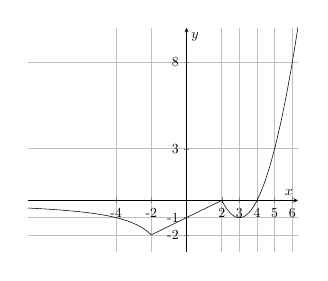
\begin{tikzpicture}[scale=0.5]
\begin{axis}[
    axis lines = middle,
    grid=major,
    legend pos={south west},
    xlabel = {$x$},
    %xlabel style={below right},
    ylabel = {$y$},
    ymin=-3,
    ymax=10,
    xtick={-4, -2, 2, 3, 4,5,6},
    xticklabels={-4, -2, 2, 3, 4,5,6},
    ytick={-2,-4 , -1 , 3, 8},
    yticklabels={-2,-4 , -1 , 3, 8},
                  ]
	\addplot[domain=-9:-2, samples=100, color=black] {4/x};
    \addplot[domain=-2:2, samples=100, color=black] {x/2-1};
    \addplot[domain=2:9, samples=100, color=black] {x*x-6*x+8};
\end{axis}
\end{tikzpicture}$$
По графику определим ответ: $m\in(-2;-1)\cup\{0\}.$\\
